%% Adaptado a partir de :
%%    abtex2-modelo-trabalho-academico.tex, v-1.9.2 laurocesar
%% para ser um modelo para os trabalhos no IFSP-SPO

\documentclass[
    % -- opções da classe memoir --
    12pt,               % tamanho da fonte
    openright,          % capítulos começam em pág ímpar (insere página vazia caso preciso)
    %twoside,            % para impressão em verso e anverso. Oposto a oneside
    oneside,
    a4paper,            % tamanho do papel. 
    % -- opções da classe abntex2 --
    %chapter=TITLE,     % títulos de capítulos convertidos em letras maiúsculas
    %section=TITLE,     % títulos de seções convertidos em letras maiúsculas
    %subsection=TITLE,  % títulos de subseções convertidos em letras maiúsculas
    %subsubsection=TITLE,% títulos de subsubseções convertidos em letras maiúsculas
    % Opções que não devem ser utilizadas na versão final do documento
    %draft,              % para compilar mais rápido, remover na versão final
    %MODELO,             % indica que é um documento modelo então precisa dos geradores de texto
    %TODO,                indica que deve apresentar lista de pendencias 
    % -- opções do pacote babel --
    english,            % idioma adicional para hifenização
    brazil              % o último idioma é o principal do documento
    ]{ifsp-spo-inf-ctds}

        
% ---

% --- 
% CONFIGURAÇÕES DE PACOTES
% --- 
%\usepackage{etoolbox}
%\patchcmd{\thebibliography}{\chapter*}{\section*}{}{}


% ---
% Informações de dados para CAPA e FOLHA DE ROSTO
% ---
\titulo{"Portal de vagas de estágio"}

% Trabalho individual
%\autor{JOSÉ BRAZ DE ARAUJO}

% Trabalho em Equipe
% ver também https://github.com/abntex/abntex2/wiki/FAQ#como-adicionar-mais-de-um-autor-ao-meu-projeto
\renewcommand{\imprimirautor}{
\begin{tabular}{lr}
Bruna da Silva Pires & SP3056651 \\
Daniel Roberto Pereira & SP3046702 \\
Igor Nathan de Oliveira Rocha & SP305263X \\
Leonardo Marques da Silva & SP3052591 \\
Lucas Lima de Santana & SP3046559 \\
Marcelo Carlos Olimpio Junior &SP3046583 \\
\end{tabular}
}


\tipotrabalho{Projeto da Disciplina PI1A5}

\disciplina{PI1A5 - Projeto Integrado I}

\preambulo{Proposta de projeto para disciplina PI1A5}

\data{2022}

% Definir o que for necessário e comentar o que não for necessário
% Utilizar o Nome Completo, abntex tem orientador e coorientador
% então vão ser utilizados na definição de professor
\renewcommand{\orientadorname}{Professor:}
\orientador{Carlos Henrique Veríssimo Pereira}
%\renewcommand{\coorientadorname}{Professor:}
%\coorientador{NOME COMPLETO DO PROFESSOR2}



% ---



% ---
% Configurações de aparência do PDF final


% informações do PDF
\makeatletter
\hypersetup{
        %pagebackref=true,
        pdftitle={\@title}, 
        pdfauthor={\@author},
        pdfsubject={\imprimirpreambulo},
        pdfcreator={LaTeX with abnTeX2},
        pdfkeywords={abnt}{latex}{abntex}{abntex2}{trabalho acadêmico}, 
        colorlinks=true,            % false: boxed links; true: colored links
        linkcolor=blue,             % color of internal links
        citecolor=blue,             % color of links to bibliography
        filecolor=magenta,              % color of file links
        urlcolor=blue,
        bookmarksdepth=4
}
\makeatother
% --- 

% ---

% ----
% Início do documento
% ----
\begin{document}

% Retira espaço extra obsoleto entre as frases.
\frenchspacing 

\pretextual

% ---
% Capa - Para proposta a folha de rosto é suficiente pois é mais completa.
% ---
\imprimirfolhaderosto
\newpage

% ---
% inserir lista de abreviaturas e siglas
% ATENCAO o SHARELATEX/OVERLEAF GERA O GLOSSARIO SOMENTE UMA VEZ
% CASO SEJA FEITA ALGUMA ALTERAÇÃO NA LISTA DE SIGLAS É NECESSARIO UTILIZAR A OPÇÃO :
% "Clear Cached Files" DISPONIVEL NA VISUALIZAÇÃO DOS LOGS 
% ---
% https://www.sharelatex.com/learn/Glossaries

\ifdef{\printnoidxglossary}{
    \printnoidxglossary[type=\acronymtype,title=Lista de abreviaturas e siglas,style=siglas]
    \cleardoublepage
}{}

% ---
% inserir o sumario
% ---
%\pdfbookmark[0]{\contentsname}{toc}
\tableofcontents*
\cleardoublepage
% ---
% ----------------------------------------------------------
% ELEMENTOS TEXTUAIS
% ----------------------------------------------------------
\textual

% ----------------------------------------------------------
% Introdução
% ----------------------------------------------------------
\chapter[Introdução]{Introdução}

%Colocar algum texto aqui, não deixar em branco

\section{Justificativa}
%O problema encontrado

\section{Proposta de solução}
%Descrição geral da nossa proposta
O Portal de vagas de estágio é um sistema para aproximar novos profissionais/estudantes da área de TI e empresas com vagas de estágio/trainee disponíveis, de modo que os candidatos possam receber indicações de vagas condizentes com seu perfil e empresas recebam recomendações de candidatos possivelmente adequados às vagas anunciadas.

\section{Objetivos}
O objetivo principal da nossa solução é promover um meio de conexão mais direto entre os estudantes em busca de estágio e empresas que buscam interessados em suas vagas de estágio alinhados com o perfil buscado. Através do sistema de recomendações, tantos os estudantes quanto as empresas têm papel ativo no processo de encontrar um(a) estudante/vaga ideal, cujas as competências e perfil sejam condizentes com o que é procurado.

A partir do nosso objetivo principal, podemos listar alguns objetivos mais práticos da nossa solução:
%Eu acho que esses itens são os requisitos funcionais, não?
\begin{itemize}
	\item Realizar o gerenciamento de vagas entre os candidatos e as empresas de uma forma simplificada;
	\item Recomendar vagas para estudantes, empresas para estudantes, estudantes para vagas/empresas;
	\item Manter um histórico de vagas aplicadas pelo estudante;
	\item Manter um histórico de candidatos aplicados a vaga;
	\item Exibir uma linha do tempo da situação da vaga;
	\item Alertar os estudantes aplicados à vaga sobre cada mudança em seu status;
	\item Possibilitar o gerenciamento da vaga pela empresa que a registrou/publicou;
	\item Possibilitar que a empresa possas acionar (entrar em contato) com os estudantes recomendados/aplicados à vaga;
	\item Possibilitar que a empresa realize mudanças no status da vaga;
\end{itemize}
	


% Para facilitar a manutenção é sempre melhore criar um arquivo por capitulo, para exemplo isso não é necessário 
%% Para facilitar a manutenção é sempre melhore criar um arquivo por capitulo, para exemplo isso não é necessário 

%---------------------------------------------------------------------------------------
\chapter{Modelo Teórico e Pressupostos (ou Hipóteses) da Pesquisa}
\explicacao{Para trabalho da Pós Graduação}
\preencheComTexto




%---------------------------------------------------------------------------------------
\chapter{Métodos de Pesquisa}
\explicacao{Para trabalho da Pós Graduação}
\preencheComTexto

\section{Tipo de Pesquisa}
\preencheComTexto

\section{Plano Amostral (se Pesquisa Quantitativa)}
\preencheComTexto

\section{Instrumento de Pesquisa e Escalas Utilizadas (Escalas se Pesquisa Quantitativa)}
\preencheComTexto

\section{Coleta de Dados}
\preencheComTexto

\section{Análise de Dados}
\preencheComTexto


%---------------------------------------------------------------------------------------
\chapter{Resultados da Pesquisa}
\explicacao{Para trabalho da Pós Graduação}
\preencheComTexto

\section{Assunto 1}
\preencheComTexto

\section{Assunto 2}
\preencheComTexto

\section{Assunto 3}
\preencheComTexto

\section{Discussão dos Resultados Observados}
\preencheComTexto

%---------------------------------------------------------------------------------------





\chapter{Requisitos}

\section{Requisitos Funcionais}

\section{Requisitos Não-funcionais}

\section{Regras de Negócio}
\chapter{Processos modelados}
% Precisamos colocar isso agora msm?
\section{Recomendação de vagas para o estudante}
\subsection{Descrição}

\subsection{Diagrama BPMN}


\section{Recomendação de estudantes para vagas cadastradas}
\subsection{Descrição}

\subsection{Diagrama BPMN}


\section{Recomendação de empresas para o estudante}
\subsection{Descrição}

\subsection{Diagrama BPMN}


\chapter{Tecnologias}
Nesse capítulo serão citadas a arquitetura do nosso projeto com ilustrações demonstrando de forma mais lúdica, as possíveis integrações que nossa aplicação terá com sistemas externos.

\section{Arquitetura}
Para o desenvolvimento do projeto, e tendo em vista que será construída uma aplicação web de página única, utilizaremos de ferramentas que cerceiam o ecossistema de \textit{Single Page Applications}. Para isso, teremos a divisão do projeto em \textit{front-end} e \textit{back-end} de modo que eles se comuniquem via protocolo HTTP com requisições e respostas no formato JSON. Para o desenvolvimento do \textit{front-end} utilizaremos Typescript por meio da biblioteca React; o \textit{back-end} será desenvolvido utilizando Java com o micro \textit{framework} Spring Boot. Um módulo de apoio no lado do servidor poderá ser possível, e para ele utilizaremos Python. 

Em relação ao deploy das aplicações, o \textit{front-end} será hospedado na plataforma Vercel, que é primariamente voltada para Javascript, proporcionando uma melhor agilidade de desenvolvimento, enquanto o \textit{back-end} será hospedado no Heroku, que é uma plataforma como serviço de fácil manuseio e que nos permitirá ter um maior foco no desenvolvimento do projeto. Através do Heroku podemos também fazer a utilização do banco de dados PostgreSQL por meio do serviço de apoio Heroku Postgres.

Ademais, se for necessário o armazenamento de objetos como arquivos ou imagens, utilizaremos a plataforma Cloudinary principalmente por sua fácil integração com a linguagem de programação Java através de bibliotecas.


\subsection{Diagramas de arquitetura}
Os diagramas \autoref{fig_arq_app}, \autoref{fig_arq_tec} e \autoref{fig_arq_negocio} ilustram de modo geral a arquitetura pensada para a solução proposta, utilizando das tecnologias já citadas.

\section{Integrações}
Nessa seção serão citadas as possíveis integrações que nossa aplicação terá, que foram decididas baseadas em outras aplicações do mercado.

\subsection{Login com o Google e LinkedIn}
Pensando na experiência de usuário, nossa aplicação terá a opção do estudante se logar através do \ac{sso} dessas empresas. Dessa forma, não será necessário digitar a senha toda vez que o usuário for usar nosso \emph{website}, precisando apenas clicar um botão e fazer o login em uma dessas alternativas.

\subsection{Entrar em contato via \emph{Whatsapp}}
Nossa aplicação terá, também, uma forma da empresa contatar o estudante via Whatsapp. Essa integração será feita via \ac{api} disponibilizada pela própria empresa que mantém o aplicativo (Meta). Dessa forma, com apenas um clique, será possível enviar uma mensagem diretamente ao estudante.

\begin{figure}[htb]
	\centering
	\caption{\label{fig_arq_app}Arquitetura de Aplicação}
	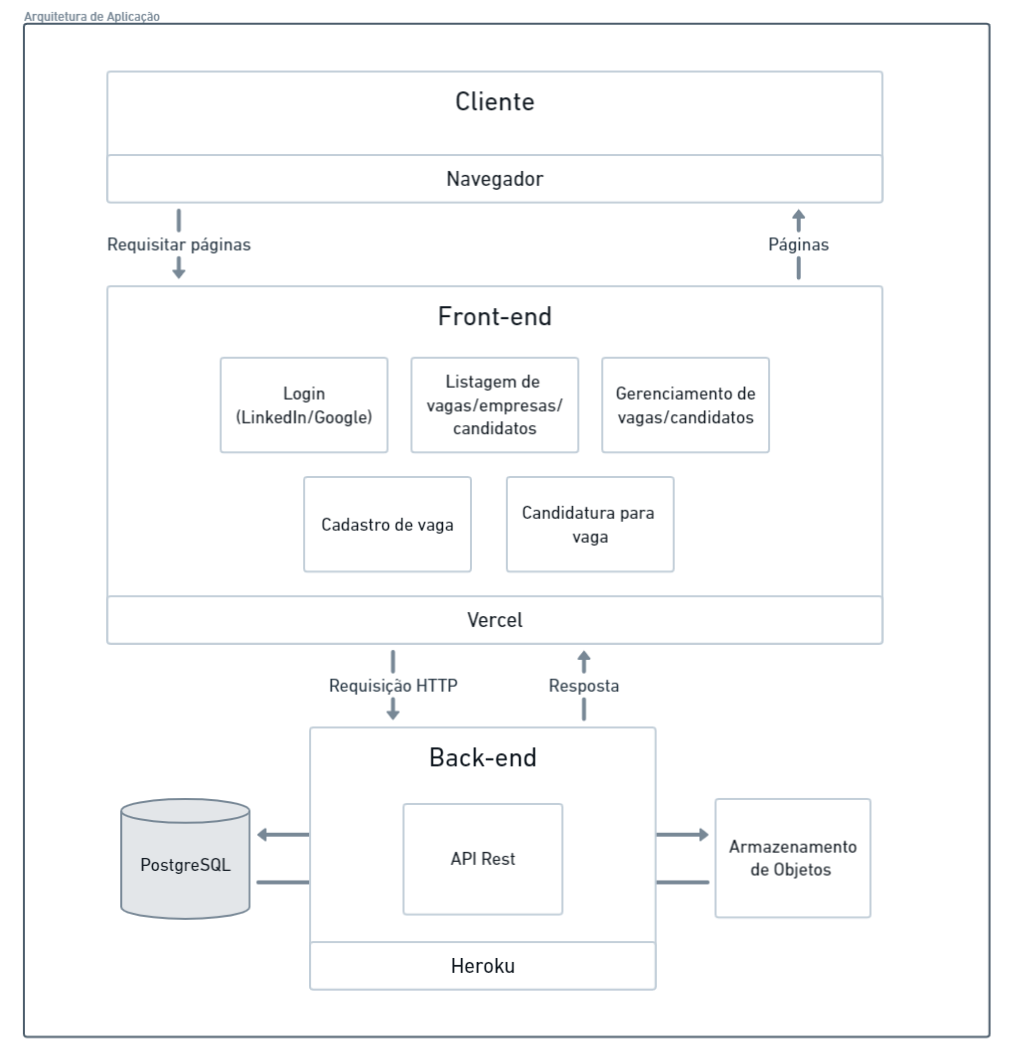
\includegraphics[width=0.95\textwidth]{imagens/arq-proj-arq-app.png}
	\fonte{Produzido pelos autores utilizando a ferramenta \textit{Whimscal}}
\end{figure}

\begin{figure}[htb]
	\centering
	\caption{\label{fig_arq_tec}Arquitetura Tecnológica}
	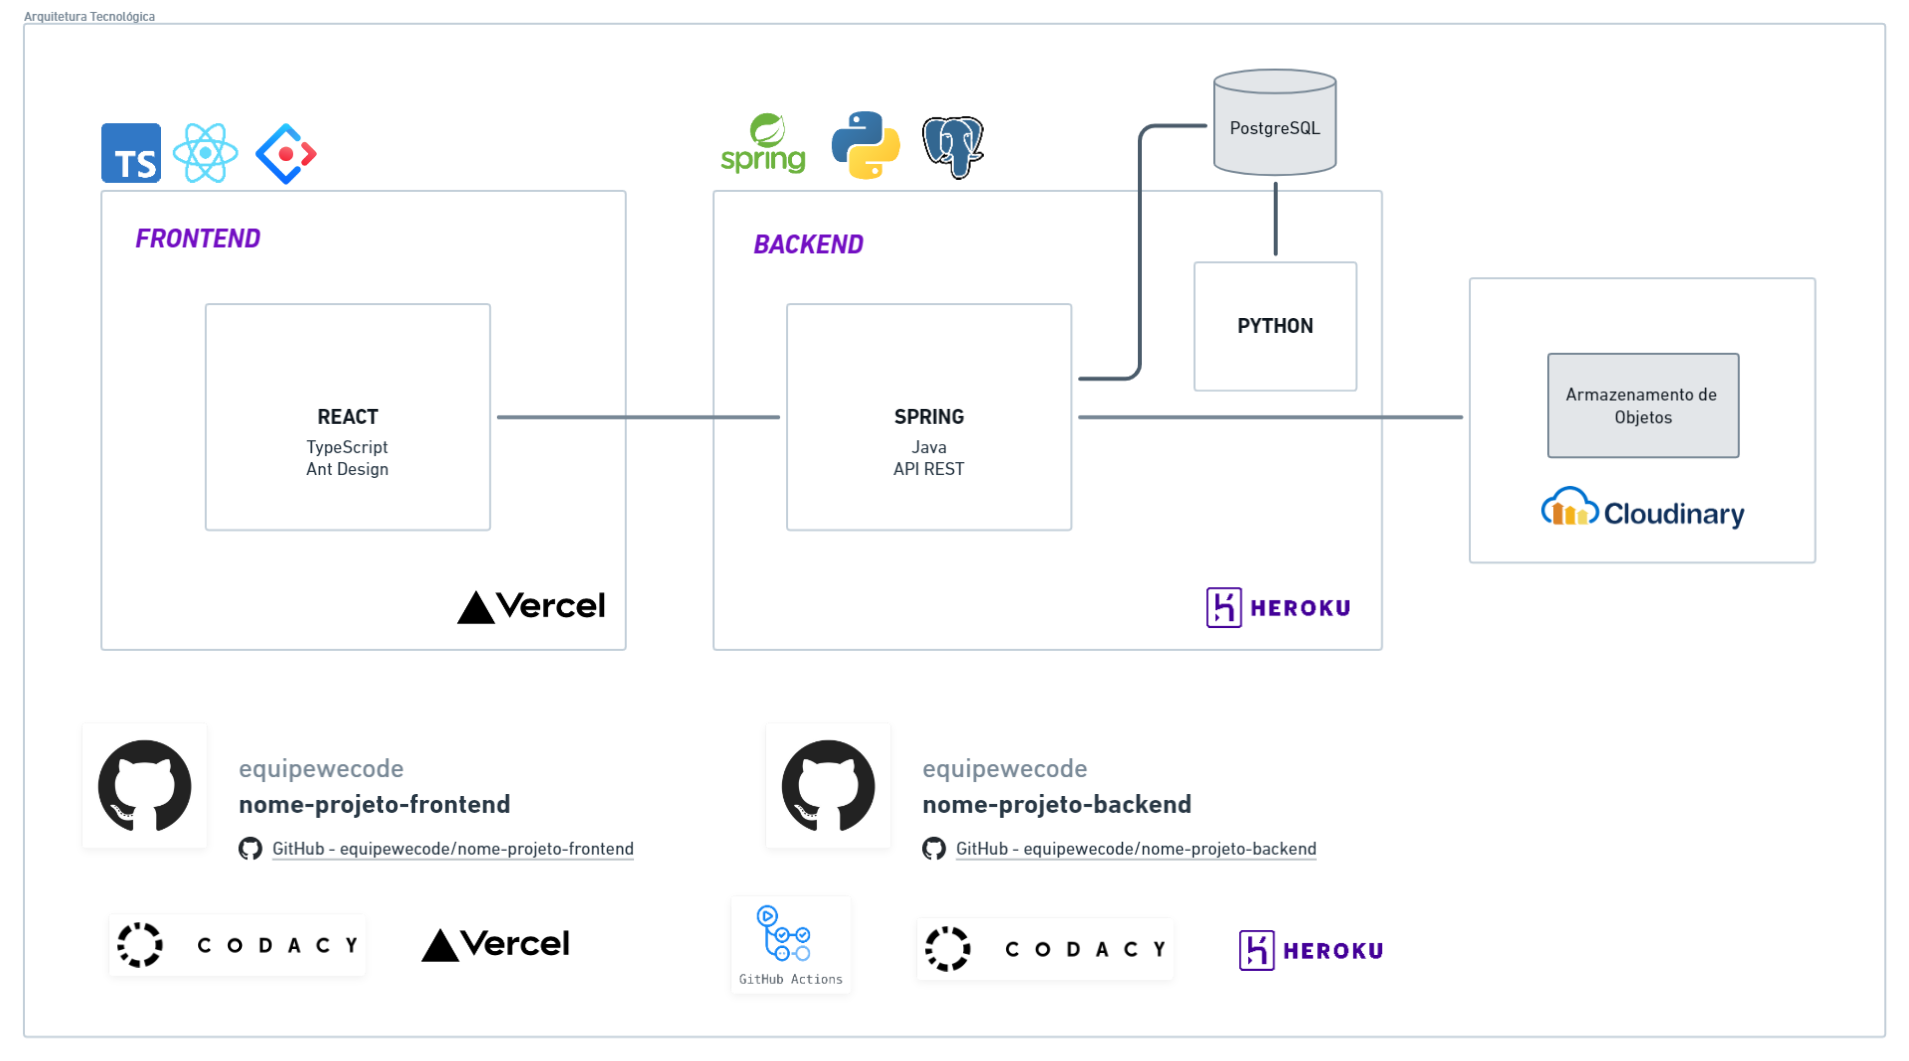
\includegraphics[width=0.95\textwidth]{imagens/arq-proj-arq-tec.png}
	\fonte{Produzido pelos autores utilizando a ferramenta \textit{Whimscal}}
\end{figure}

\begin{figure}[htb]
	\centering
	\caption{\label{fig_arq_negocio}Arquitetura de Negócios}
	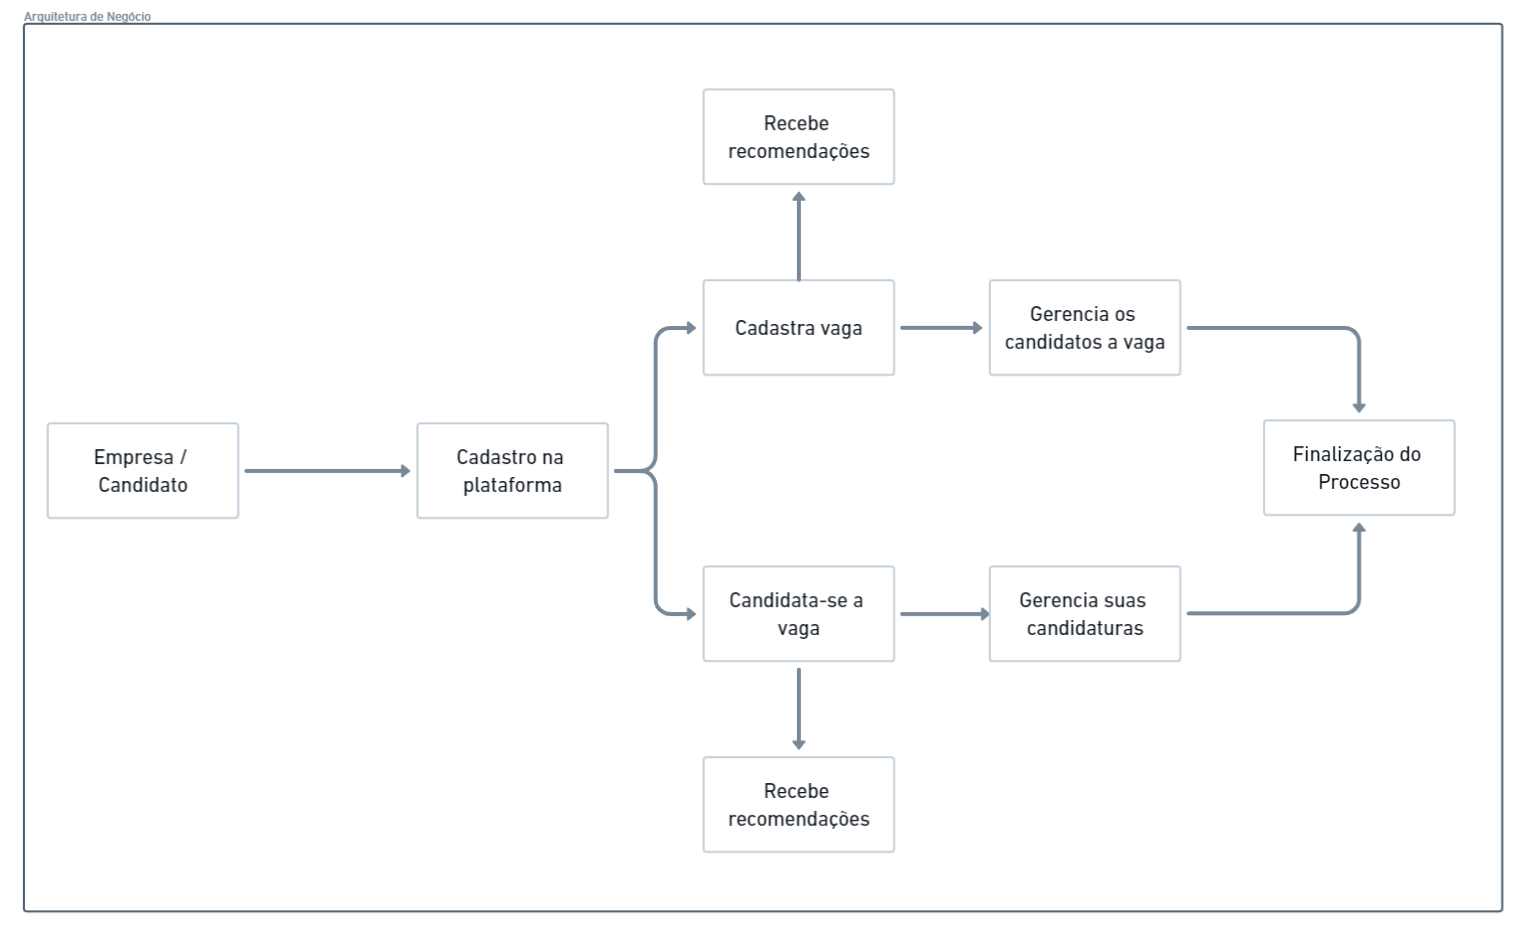
\includegraphics[width=0.95\textwidth]{imagens/arq-proj-arq-negocio.png}
	\fonte{Produzido pelos autores utilizando a ferramenta \textit{Whimscal}}
\end{figure}

%% ---
% Conclusão (outro exemplo de capítulo sem numeração e presente no sumário)
% Dependendo do trabalho desenvolvido ele pode ter uma Conclusão ou Considerações finais
% Para trabalhos de disciplina utilizar Considerações Finais
% ---
\chapter{Considerações Finais}
% Exemplo de como adicionar linha adicional no sumário
%\addcontentsline{toc}{chapter}{Considerações Finais}
% Para definir sem número utilizar o asterisco
% Mas se tiver sub seção vai continuar a contagem do capítulo anterior
%\chapter{Considerações finais}



% ---
Além desse documento ser um modelo de como pode ser criado um documento em \LaTeX \space ele também apresenta diversas informações úteis para as disciplinas de projetos de informática do \ac{ifsp} e alguns elementos uteis para as monografias do curso de Pós Graduação em Gestão de \acs{ti} do \ac{ifsp}.

\explicacao{Um trabalho de disciplina não tem \enquote{Conclusão}}

\preencheComTexto


\explicacao{Exemplo de possíveis seções para monografia da pós graduação...}
\section{Resposta à Questão de Pesquisa}
\preencheComTexto

\section{Objetivos Propostos}
\preencheComTexto

\section{Contribuições Acadêmicas e Gerenciais}
\preencheComTexto

\section{Limitações da Pesquisa e Contribuições para Estudo}
\preencheComTexto



%Teste de citação para gerar referências no modelo.. \citeauthor{SCRUMGUIDE:2013}


% ----------------------------------------------------------
% Referências bibliográficas
% ----------------------------------------------------------
%\bibliography{referencias,exemplos/abntex2-doc-abnt-6023}

\end{document}